\subsubsection{配列構造}
配列を複数定義し,一つの計算の中で呼び出す場合空間的局所性が低くなり,キャッシュミスを多く生じさせる可能性がある.
そのため,同時に利用する配列達を一つの配列としてくくりだすことで空間的局所性を高くし,高速化を図る手法が考えられる.\\
{\footnotesize
\begin{lstlisting}[numbers=none]
int a[100], b[100], c[100], d[100];
for i=0 to 100 {
  d[i] = a[i] + b[i] + c[i];
}
\end{lstlisting}
}
というプログラムを例とすると,
{\footnotesize
\begin{lstlisting}[numbers=none]
int abcd[100][4];
for i=0 to 100 {
  abcd[i][3] = abcd[i][0] + abcd[i][1] + abcd[i][2];
}
\end{lstlisting}
}
とすることで連続した領域にアクセスさせることができるようになり,キャッシュ効率の向上が見込まれる.\\
一方で,SIMD化の観点では配列の各要素がバラバラになってしまい非連続的になるためSIMD命令を使いにくくなる可能性もある.\\

\begin{figure}[htb]
% h:here, t:top, b:bottom, p:page
  \begin{center}
    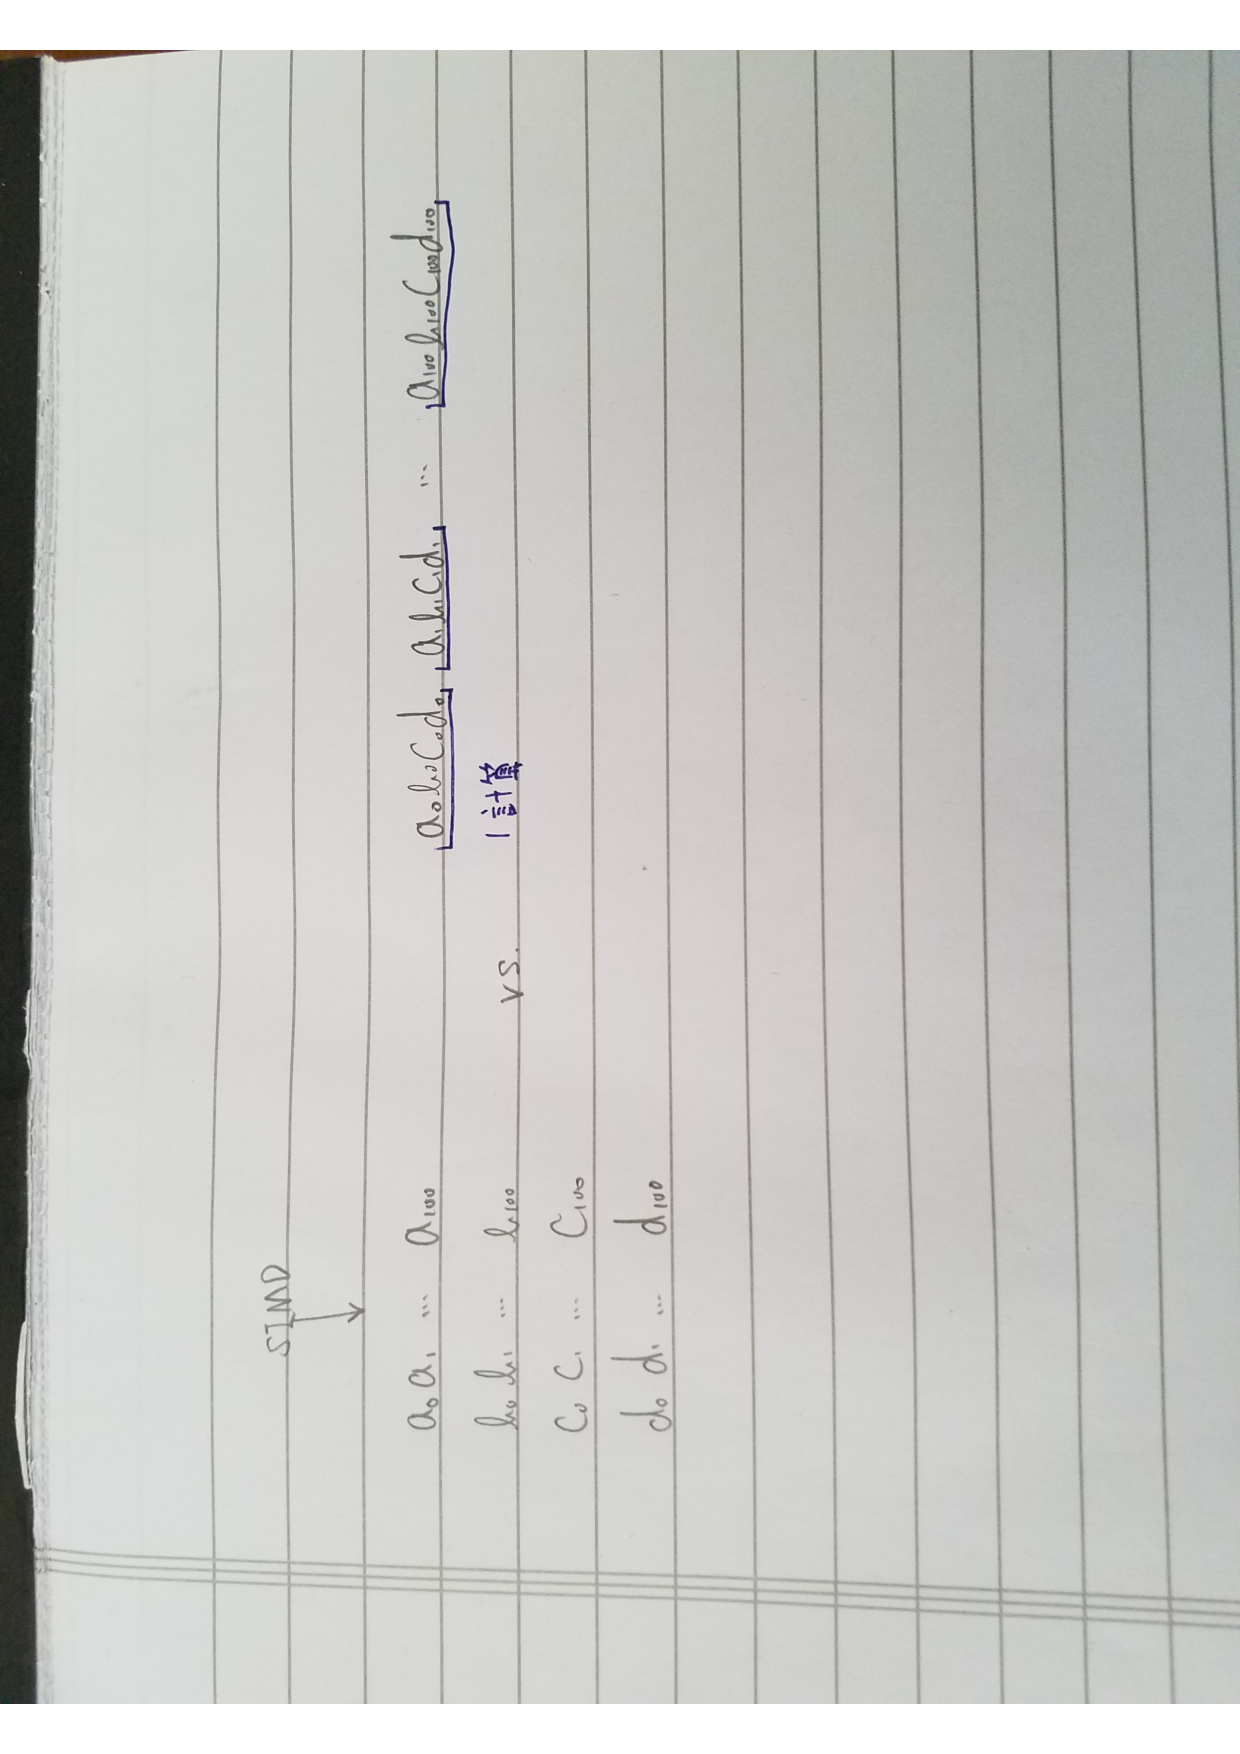
\includegraphics[width=10.0cm, angle=-90]{./images/simd_soa.pdf}
    \caption{SIMD化と配列のくくりだし}
    \label{fig:simd-soa}
  \end{center}
\end{figure}~\\
以上から空間局所性とSIMD化という最適化を行う上で大変重要な要素どちらか一方だけを考えるのではなく,
適切なハイブリッド構造を用いることを目指した.\\
( TODO: 事実確認)
演算に利用する変数の数が多い時はSIMD化は難しい. これはSIMD演算器のビット数に依存する問題だが倍精度の演算をする場合
1-4変数(double型64bitsに対しSIMD演算器は64-256bitsが一般的)の演算を並列処理できるが,変数の数がより多い場合は
同時に実行することが不可能であるからである.\\
この場合,配列をくくり出すことによって空間局所性を高くする方がより計算処理の高速化を実現できると考えられる.\\
また,配列をくくり出す際相互に関係のない配列を一つにまとめてもキャッシュラインに入りきらなくなるなどの問題が発生する.\\

以上を踏まえ,SIMD化と配列のくくりだしのハイブリッドを実現するために以下のアルゴリズムを実装した.\\
{\footnotesize
\lstinputlisting[caption=SIMD化と配列のくくりだしのアルゴリズム 疑似コード,label=pseudocode-simd-soa,frame=single]{src/pseudocode/simd-soa}
}~\\

\paragraph{Union-Find木の利用}~\\
MODファイル内で
\begin{eqnarray}
  a &=& b * c\\
  d &=& e * f\\
  g &=& a + h
\label{eq:3x0}
\end{eqnarray}
と記述されていたとすると,各ステップの計算において関連しうる変数は(a, b, c, g, h)と(d, e, f)であることがわかる.\\
そのため,相互に関連しえない変数に関しては互いに影響を及ぼさないため,
グループとしてまとめ切り離して考えることができる.\\
このグループを作成するにあたり,Union-Find木を用いてMODファイルに定義された式の変数を分類した.\\
こうしてUnion-Find木で作成されたグループは,空間局所性またはSIMD化のどちらかがより有効に働くことから,
それぞれのグループを配列としてくくり出すか否かを独立に試行することで空間局所性とSIMD化のハイブリッドを
実現することができると考える.\\
よって,仮に変数のグループがn個できた場合でも2n回の試行を行うことで最適な組み合わせを見つけることができる.
( TODO: 論文を引用)
